\documentclass{vie16}
\usepackage{wrapfig}
\usepackage{float}
\usepackage{amsmath}
\usepackage[table,xcdraw]{xcolor}
\usepackage{booktabs}
\usepackage{multirow}
\usepackage{adjustbox}

% Path to figures
\graphicspath{{Fig/}}

% COMENTAR ANTES DE SUBMETER!
% Comando temporarios
\usepackage{color}
\usepackage[normalem]{ulem}
\newcommand{\new}[1]{\textcolor{blue}{#1}}
\newcommand{\old}[1]{\textcolor{MyDarkViolet}{\sout{#1}}}
\newcommand{\att}[1]{\textcolor{red}{#1}}
\newcommand{\js}[1]{\textcolor{darkgreen}{#1}}
\newcommand{\obs}[1]{\textcolor{orange}{#1}}
\definecolor{MyDarkViolet}{rgb}{0.602,0,0.602}
\definecolor{orange}{RGB}{255,127,0}
\definecolor{darkgreen}{RGB}{0,127,0}

% For pdf hyperlinks
\usepackage{hyperref}
\hypersetup{colorlinks=true}
\hypersetup{citecolor=blue}
\hypersetup{pdftitle={Development of lock-in resistivimeter
for measuring resistivity and induced polarization under
high electrical noise}}
\hypersetup{pdfauthor={J.~M.~Oliveira, W.~C.~Ferreira and F.~Hiodo}}
% For making a print without color links
\hypersetup{linkcolor=black,citecolor=black,filecolor=black,urlcolor=black}
\hypersetup{linkcolor=blue,citecolor=blue,filecolor=blue,urlcolor=blue}
\usepackage{url}
\begin{document}

\title{Development of lock-in resistivimeter for measuring
resistivity and induced polarization under high electrical noise}
\author{J.~M.~Oliveira, W.~C.~Ferreira and F.~Hiodo}
\maketitle

% Nota: geralmente a EAGE limita o numero de caracteres no abstract. 

\begin{abstract}

	The Cole-Cole RC circuit model and the reduced clay model were
	tested with three levels of white noise in order to develop a low
	cost lock-in resistivimeter. The device has maximum power of 60
	watts and showed reliable stability under $67 \%$ and $11 \%$ of
	white noise in the respective models. The equipment was made with
	low cost components and yet capable of providing a frequency sweep
	from $13$ to $120$Hz to the transmitter which allows better signal
	sampling. The viability of this frequency bandwidth for application in
	Spectral Induced Polarization (SIP) were also studied using the
	Cole-Cole equation. This model was used to find the less time
	consuming operational settings able to recover the Cole-Cole
	exponent and relaxation time, in other words, which are the minimum
	number of frequency samples that is necessary to reconstruct the
	Cole-Cole curve. An inversion scheme based on the partial sweep of
	the solution space was implemented. We found that $16$ frequency
	samples evenly spaced are enough to recover the relaxation time with
	variations below one order of magnitude. Therefore, the results
	showed good performance for the developed lock-in resistivimeter.
	The suggested applications to such equipment is not only restricted
	to field measurements but also to lab samples studies related to
	Spectral Induced Polarization (SIP), resistivity and Induced
	Polarization (IP) under high electrical noise.  
\end{abstract}	
		

\newpage


\section{Introduction}
Urban regions are characterized by a high noise content to the
geoelectrical methods mainly due to presence of power supply,
grounding and stray voltages. It's also known that intrusive methods
are affected by pavimentation and buildings which impose restrains in
the superficial area making them more susceptible to noise. The
objectives of this work is the design of a synchronous detection
resistivimeter from low cost components to conduct resistivity and IP
surveys using low power supply.  As observed in Figure 1 the equipment
basically consists of a transmitter and a receiver with two channels
each. The reference channel is fed directly in the receiver while the
signal channel is injected from the transmitter into the subsurface
and then to the receiver. An ideal lock-in transmitter would have an
infinite frequency sweep without any distortion and would deliver
constant power for all frequencies. However, due to physical
limitation our transmitter is capable to provide a stable power supply
close to 60W for the frequency bandwidth of 13 to 120Hz with minimal
distortion.  Bellow the 13Hz threshold the electrical sine wave
distortion increases drastically and above the 120Hz there is little
gain of information due to logarithmic nature of frequency.

\section{Sincronous Detection}
As introduced by \citet{meade13} the synchronous detection also known
as \textit{lock-in} is sensitive to the differences in frequency and
phase between two input signals.  Inside the receiver, the reference
channel is converted to an unitary square wave to multiply the
demodulated signal of interest. As shown in the complete scheme of
Figure \ref{f:Lock-in}, after the multiplication the product goes
into a low-pass filter. Setting the cut off frequency of the low-pass
filter to a value no greater than the reference frequency will produce
the output to be a DC voltage signal described by equation \ref{e:v_out}.

\begin{equation}
	v_{(t)} = H_{(\omega)} V_{S} 
									\cos \left(
												\phi_{R} - \phi_{S}
										 \right)
						+
				H_{(\omega)} {\langle n_{(t)} \rangle}_{\lambda}
	\label{e:v_out}
\end{equation}

where $H_{(\omega)}$ is a transfer function of the low-pass filter,
$V_{S}$ and $\phi_{S}$ are the amplitude and phase of the measured
signal, $\phi_{R}$ is the phase of the square wave and ${\langle
	n_{(t)} \rangle}_{\lambda}$ is the noise averaged over the time of
	measurement $\lambda$. 

% Se puder falar do filtro usado ia ser muito bom. 

\begin{figure}[H]
	\centering
	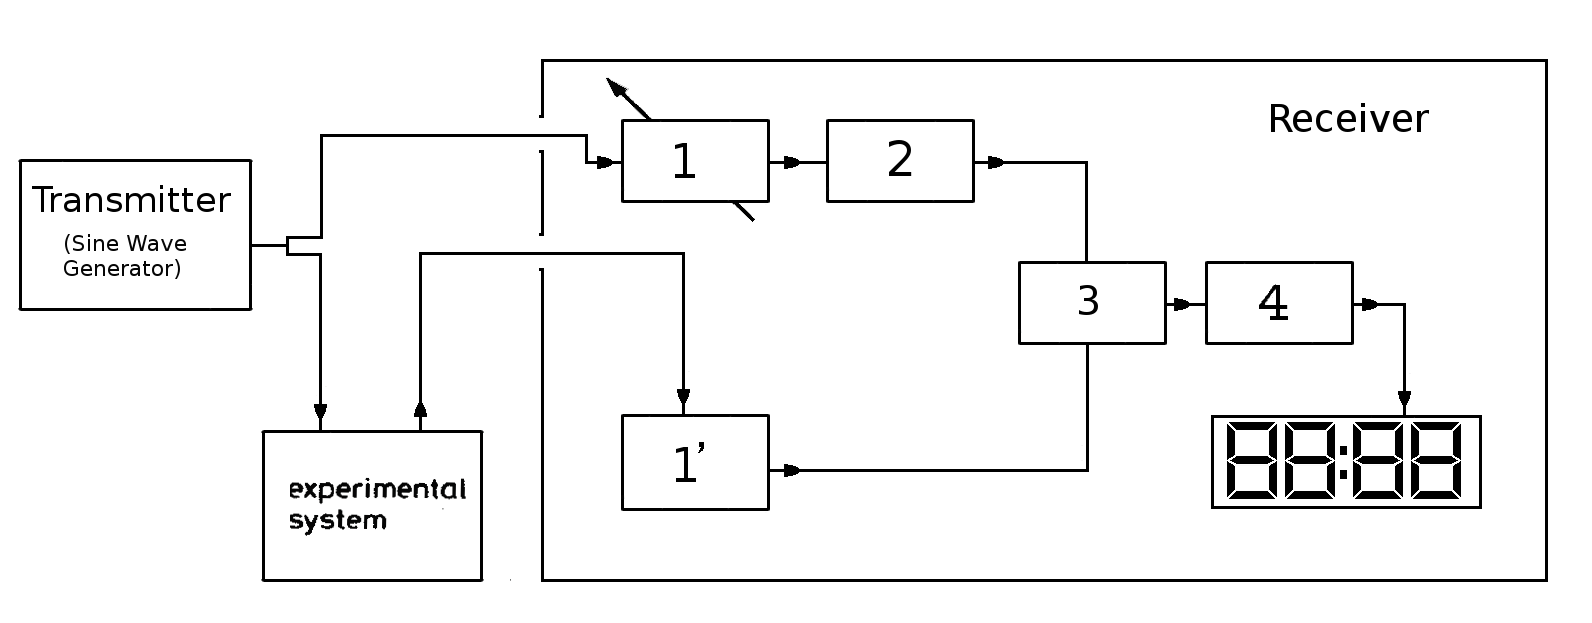
\includegraphics[keepaspectratio=true,scale=0.3]{Sistema-Inside_Lock_In}
	\caption{Scheme of synchronous detection. The arrows show the way followed by the source signal from the transmitter injected into the receiver reference channel (\textit{up}) and signal channel (\textit{down}). In the signal channel $1^{,}$ there is a optional amplifier or attenuator. In the reference channel $1$ is a phase-shifter for correcting the added phase from the detector, $2$ output a square wave from the sine wave input, $3$ is the multiplier and  $4$ the low-pass filter led to the display. }
	\label{f:Lock-in}
\end{figure}


The main advantage of the lock-in resistivimeter over convetional ones
(DC) is illustrated in equation \ref{e:v_out} by the attenuation of
noises such as the white noise whose phase doesn't correlate with the
reference signal since it's average over time approaches zero. The
Johnson-Nyquist noise is perhaps the most significant in geoelectrical
measurements since it's amplitude increases with the spacing of the
geoelectrical arrays \citep{alfano82}.

Setting a narrow bandwidth filter is possible to avoid almost all
interferences including the electric power supplies which can be
avoided in our multifrequency resistivimeter by sampling the data in
another frequency far from 55Hz - 60Hz.

There are two possible configurations for taking measurements: (1)
Setting $\phi_{R}$ in-phase with $\phi_{S}$ and (2) Setting $\phi_{R}$
in quadrature with $\phi_{S}$. Using the configuration (1) the
resistivimeter is sensible only to amplitude $V_{S}$ changes while in
(2) it works linearly with changes in phase $\phi_{S}$ until the phase
of ${\pi}/{6}$rad. Both measurements can be used to extract
information of capacitive and resistivity properties of the subsurface
as discussed by \citet{tarasov13},\citet{edmundo14} and
\citet{weller96}.

\section{Inversion}
Due to practical limitations, our resistivimeter works in frequencies
ranging from $13$ to $120$Hz. However, we still investigate the
viability to use this equipment to perform Spectral Induced
Polarization (SIP) studies. Therefore an inversion scheme of the
Cole-Cole parameters was used to verify how many frequency samples in
this range were needed to re-build the Cole-Cole curve. The
implemented technique was the partial sweep scheme, it consists of
choosing specific values for the relaxation time ($\tau$) and for the
Cole-Cole exponent ($c$) inside a prior established interval and then
computing a \textit{l2-norm} between each modelled curve and the data.
In the last step, it's built an map of the solution space which is
analized to look for the minima positions.  Using equation \ref{e:CC}
, defined by \citet{tarasov13} we define $c \in [0:1]$ and $\tau \in
[10^{-4}:10^{4}]$ based on empirical values for relaxation time
\citet{telford90} . It is important to highlight that we could have
more than one relaxation time in the data, however to simplify our
analysis only one relaxation time (with possible values inside the
prior defined range) is used for each Cole-Cole curve.


%    Smith, M.J., 1980, Comparison of induced polarization measurements over the Elura orebody, The Geophysics of the Elura Orebody, Cobar NSW, ASEG, 1980, 77-80.

\begin{equation}
	\sigma_{e} = \sigma_{0}
			\left[
			1 + \frac{m}{1-m}
						\left( 
								1 - \frac{1}{1+ \left( j\omega\tau \right)^{c} }	
						\right) 			
			\right]
	\label{e:CC}
\end{equation}

where $\sigma_{e}$ is the complex conductivity, $\sigma_{0}$ is the
conductivity at zero frequency, $m$ is the chargeability, $\omega$ is 
the angular frequency, $\tau$ is the relaxation time and $c$ is the 
Cole-Cole exponent.


\section{Results}


% transfer function do equipamento
% synchronous detection baixa deriva termica, experimento
% durou horas

% Eu até posso calcular. Dependendo de quantas folhas sobrarem.
%Chargeability could be found from the measured data by the equation 
%\begin{equation}
%	F_{E} = \frac{ |V_{(\omega_{1})} - V_{(\omega_{2})}| }{V_{(\omega_{1})}}
%	\label{e:FE}
%\end{equation}


In order to verify the performance of the equipment in noisy
environments, was conducted an experiment with scaled models testing
how much of the measurements are affected by white noise. The results
of Table \ref{t:scaled_models} show a good performance even under
$67\%$ in the RC circuit of $12 \mu$F. As the result of such high
capacitance, the in-phase and the quadrature measurements were
switched. The outcome of a model more similar to the expected data
from field surveys was also used. A clay tank of $1125$ cm$^3$, also
points to application even under $11\%$ of white noise as showed in
Table \ref{t:scaled_models}.

\begin{table}[H]
\centering
\caption{Measured voltage on scaled models with three levels of white noise.}
\label{t:scaled_models}
\begin{tabular}{cccl|ccc}
\multirow{2}{*}{\textbf{Noise level (\%)}}  & \multicolumn{2}{c}{\textbf{Output}}     &  & \textbf{Noise Level (\%)} & \multicolumn{2}{c}{\textbf{Output}}     \\
                         & \textbf{In Phase}  & \textbf{Quadrature} &  &  	 				& \textbf{In Phase} & \textbf{Quadrature} 	\\
\multirow{4}{*}{0}	 		& 1.52              & 8.45                &  & 	\multirow{4}{*}{0}	&  5.24				&		1.80			\\
					 		& 1.60              & 8.50                &  &						&  4.75				&		1.90			\\
					 		& 1.44              & 8.46                &  &						&  4.80				&		1.92			\\
					 		& 1.48              & 8.40                &  &						&  5.30		    	&		1.81	 
                                         \\ \hline                                   
\multirow{4}{*}{40}	 		& 1.06              & 8.42                &  & 	\multirow{4}{*}{11}	&	4.70			&		1.32			\\
					 		& 1.28              & 8.41                &  &						&	4.60			&		1.20			\\
					 		& 1.29              & 8.37                &  &						&	4.68			&		1.26			\\
					 		& 1.30              & 8.45                &  &						&	4.50			&		1.28			  
                                         \\ \hline
\multirow{4}{*}{67}	 		& 1.29              & 8.48                &  & 	\multirow{4}{*}{27}	&	2.30			&		1.30			\\
					 		& 1.28              & 8.48                &  &						&	2.05			&		1.20			\\
					 		& 1.29              & 8.48                &  &						&	2.12			&		1.24			\\
					 		& 1.30              & 8.50                &  &						&	2.50			&		1.32			  
                                          \\ \hline
\end{tabular}
\end{table}

As for the Cole-Cole paramenters, the effect of noise and of sample
interval were tested for three different models using four values of
Gaussian noise and to four different frequency sampling at $5\%$ of
Gaussian noise respectively. For these three models, the frequency for
theirs relaxation time are not inside the frequency bandwidth of the
resistivimeter. Therefore, the characteristic Cole-Cole curve can't be
observed. In this way, the measured data approach a straight line. 

As we can see in Table \ref{t:INV-noise_effect}, the exponent of
Cole-Cole was very well determinated for all cases, even under $250\%$
of noise, despite relating a dependence of complex conductivity with
frequency as showed in the original work of \citet{cole41}.

In other hand the relaxation time is strongly affected by noise. In Table \ref{t:INV-noise_effect} we can see that it's precision vary with the 
percent of noise while it's accuracy stay roughly the same with the exception of the most extreme case of $250\%$ of noise. Nonetheless the best 
results of all models recover both parameters within $10\%$ of uncertainty supporting it's application for SIP.

\begin{table}[H]
\centering
\caption{Noise effect on the inversion of Cole-Cole parameters}
\label{t:INV-noise_effect}
\begin{tabular}{@{}|c|c|c|c|c|c|c|@{}}
\multicolumn{3}{|c|}{\textbf{Sinthetic Model}}                             & \multirow{2}{*}{\textbf{\begin{tabular}[c]{@{}c@{}}Noise\\ (\%)\end{tabular}}} & \multicolumn{3}{c|}{\textbf{Calculated Model}}                            \\
\textbf{Model}     & \textbf{$\tau$}          & \textbf{$e_{cc}$}          &                                                                                & \textbf{$\tau$} & \textbf{$e_{cc}$} & \textbf{$\tau$ deviation}           \\  \hline
\multirow{4}{*}{A} & \multirow{4}{*}{567.243} & \multirow{4}{*}{0.0452261} & 5                                                                              & 567.243         & 0.0452261         & 567 \textless$\tau$\textless 860    \\
                   &                          &                            & 10                                                                             & 517.092         & 0.0452(5)         & 113 \textless$\tau$\textless 3405   \\
                   &                          &                            & 25                                                                             & 517.092         & 0.045(1)          & 56 \textless$\tau$\textless 5670    \\
                   &                          &                            & 250                                                                            & 517.092         & 0.045(2)          & 170 \textless$\tau$\textless 11344  \\ \hline
\multirow{4}{*}{B} & \multirow{4}{*}{2.89942} & \multirow{4}{*}{0.0452261} & 5                                                                              & 2.89942         & 0.0452(5)         & 1.15 \textless$\tau$\textless 11.6  \\
                   &                          &                            & 10                                                                             & 2.89942         & 0.045(1)          & 2.3 \textless$\tau$\textless 4.4    \\
                   &                          &                            & 25                                                                             & 2.89942         & 0.045(5)          & 1.8 \textless$\tau$\textless 5.8    \\
                   &                          &                            & 250                                                                            & 2.89942         & 0.04(1)           & 1.8 \textless$\tau$\textless 14500  \\ \hline
\multirow{4}{*}{C} & \multirow{4}{*}{622.257} & \multirow{4}{*}{0.834171}  & 5                                                                              & 622.257         & 0.834171          & 622.257                             \\
                   &                          &                            & 10                                                                             & 622.257         & 0.834171          & 622.257                             \\
                   &                          &                            & 25                                                                             &                 &                   &                                     \\
                   &                          &                            & 250                                                                            & 622.257         & 0.8(1)            & 435 \textless $\tau $\textless 1245
\end{tabular}
\end{table}

The number of samples needed in a survey also were studied with $5\%$ of noise, considered a bad %adverse?
field situation \citet{sandor11}. As showed in Table \ref{t:INV-sample_effect} with $16$ samples evenly distributed the relaxation 
time was within the same order of magnitude of the synthetic model. Despite being less precise, $8$ frequency samples also had similar uncertainty therefore being an viable option as well.

\begin{table}[H]
\centering
\caption{Sampling effect on the inversion of Cole-Cole parameters}
\label{t:INV-sample_effect}
\begin{tabular}{@{}|c|c|c|c|c|c|c|c|@{}}
\multicolumn{3}{|c|}{\textbf{Sinthetic Model}}                             & \multirow{2}{*}{\textbf{Sampling}} & \multicolumn{3}{c|}{\textbf{Calculated Model}}                          & \multirow{2}{*}{\textbf{Missfit}}    \\
\textbf{Model}     & \textbf{$\tau$}          & \textbf{$e_{cc}$}          &                                    & \textbf{$\tau$} & \textbf{$e_{cc}$} & \textbf{$\tau$ deviation}         &                                      \\ \hline
\multirow{4}{*}{A} & \multirow{4}{*}{567.243} & \multirow{4}{*}{0.0452261} & 2                                  & 517.092         & 0.045(1)          & 113 \textless$\tau$\textless 1702 & 0.02                                 \\
                   &                          &                            & 4                                  & 474.313         & 0.045(1)          & 454 \textless$\tau$\textless 1702 & 0.01                                 \\
                   &                          &                            & 8                                  & 567.243         & 0.0452261         & 568 \textless$\tau$\textless 850  & 0.02                                 \\
                   &                          &                            & 16                                 & 517.092         & 0.045(1)          & 453 \textless$\tau$\textless 568  & 0.03                                 \\ \hline
\multirow{4}{*}{B} & \multirow{4}{*}{2.89942} & \multirow{4}{*}{0.0452261} & 2                                  & 2.89942         & 0.045(1)          & 0.5 \textless$\tau$\textless 2.9  & 0.007                                \\
                   &                          &                            & 4                                  & 2.89942         & 0.045(1)          & 0.5 \textless$\tau$\textless 2.9  & 0.013                                \\
                   &                          &                            & 8                                  & 2.89942         & 0.045(1)          & 1.5 \textless$\tau$\textless 11.6 & 0.015                                \\
                   &                          &                            & 16                                 & 2.89942         & 0.0452261         & 2.3 \textless$\tau$\textless 2.9  & \textless $10^{-5}$                  \\ \hline
\multirow{4}{*}{C} & \multirow{4}{*}{622.257} & \multirow{4}{*}{0.834171}  & 2                                  & 622.257         & 0.834171          & 622.257                           & \multirow{4}{*}{\textless $10^{-5}$} \\
                   &                          &                            & 4                                  & 622.257         & 0.834171          & 622.257                           &                                      \\
                   &                          &                            & 8                                  & 622.257         & 0.834171          & 622.257                           &                                      \\
                   &                          &                            & 16                                 & 622.257         & 0.834171          & 622.257                           &                                   \\  \hline
\end{tabular}
\end{table}

For the inversion of Cole-Cole parameters the percent of noise in the
synthetic model was considered as being the output from ours
resistivimeter. Thus filtering capabilities of our resistivimeter
wasn't taken account. By the noise rejection displayed in Table \ref{t:scaled_models} the viability of SIP is reinforced since a high level of noise in the output consequently implying in higher level of noise in the input. 

\section{Conclusions}

Compared to others instruments in use today, the low power
resistivimeter was able to reject great amount of noise in scaled
models. The results show stable measurements up to $67\%$ of white
noise in RC circuit and $11 \%$ in the clay experiment. These results
strongly support the viabilty of such low cost device in geoelectrical
surveys even in high noise environments. The inversion study for the
Cole-Cole parameters points towards the viability of the equipment in
others applications such as the multifrequency resistivimeter for
Spectral Induced Polarization with a bandwith of $13$ to $120$Hz. We
showed that $8$ frequency samples evenly distributed were enough to
recover the Cole-Cole parameters.



%A  intensa rejei\c{c}\~ao de ru\'idos pelo m\'etodo de detec\c{c}\~ao s\'incrona permite a manufatura de eletrorresistiv\'imetros com baixo custo de mercado e baixa pot\^encia de opera\c{c}\~ao se comparado a outros equipamentos em uso no mercado. 
		
%		Este tipo de eletrorresistiv\'imetro apresentou estabilidade para at\'e $11\%$ de ru\'ido branco para as medidas da argila no modelo em escala reduzida. Este nivel de ru\'ido representa uma situa\c{c}\~ao muito desfavor\'avel para a aquisi\c{c}\~ao geoel\'etrica, mostrando que o desempenho do equipamento \'e suficientemente confi\'avel para sua aplica\c{c}\~ao em ambientes ruidosos.
		
%		Dada a possibilidade de aquisi\c{c}\~ao com v\'arias frequ\^encias, foi analisado o potencial da aplica\c{c}\~ao do eletrorresisitiv\'imetro na medida de polariza\c{c}\~ao ind\'uzida espectral. Os resultados obtidos pela invers\~ao dos par\^ametro de Cole-Cole, sugerem que a faixa de $13$ a $110$ Hertz \'e suficiente para a recupera\c{c}\~ao dos par\^ametros do modelo.
		
%		De maneira a aperfei\c{c}oar o equipamento para uso em campo, \'e sugerido a digitaliza\c{c}\~ao da sa\'ida, desta forma a fase poderia ser medida diretamente no equipamento eliminando a etapa de calibra\c{c}\~ao. Esta medida tamb\'em que os dados sejam salvos no equipamento, acelerando o seu processamento. 

\bibliography{abstract_EAGE}


\end{document} 